\documentclass[11pt,a4paper]{article}

% -------------------- Packages --------------------
\usepackage[a4paper,margin=2.5cm]{geometry}
\usepackage{graphicx}
\usepackage{float}
\usepackage{booktabs}
\usepackage{amsmath}
\usepackage{siunitx}
\usepackage{hyperref}
\usepackage{xurl}
\usepackage{enumitem}
\usepackage{caption}
\usepackage{subcaption}
\usepackage{cite}
\usepackage{tikz}

% -------------------- Title Info --------------------
\title{Control \& Automation for the Efficient Use of Energy\\(CAPUEE 25--26)}
\author{Bujin Shao \and Hemeng Wang \and Nai-Chi Cheng \and Saúl Daniel Castañeda Arzaga}
\date{December 26, 2025}

\begin{document}
\maketitle

% ==================================================
\begin{abstract}
% Concise summary: problem, approach, prototype, results, key takeaway.
\end{abstract}

\tableofcontents

% ==================================================
\newpage
\section{Introduction}

\subsection{Background \& Motivation}
% Context + why this matters (energy efficiency, safety, user guidance, dynamic pricing, etc.)

\subsection{Project Goals}
% Concise summary: problem, approach, prototype, results, key takeaway.

\subsection{System Overview of the Proposed Solution}
% High-level principle: sense (current + temperature) -> decide -> actuate + recommend schedule via price API
% Insert diagram: sensors -> ESP32 -> control logic -> actuators + data logging/UI + external API
\begin{figure}[H]
  \centering
  % \includegraphics[width=0.95\linewidth]{figures/system_flow.pdf}
  \caption{System schematic of the prototype.}
  \label{fig:system-flow}
\end{figure}

% ==================================================
\newpage
\section{Project Description \& Workflow}

\subsection{Problem Statement}
% What problem are you solving with the smart hair dryer?
Conventional household hair dryers operate largely in an open-loop fashion at the system level, with user-selected heat and airflow settings and only fixed, hardware-based thermal protection.

In addition, users exhibit significant variability in hair properties, such as hair thickness and hair porosity, which strongly influence heat absorption, moisture retention, and drying dynamics. However, conventional hair dryers apply identical thermal behavior regardless of these differences, potentially resulting in unnecessary energy consumption or increased thermal stress.

Furthermore, users lack intuitive information regarding electrical energy usage, thermal risk, and optimal drying strategies under varying environmental conditions, such as ambient temperature and humidity.

The problem addressed in this project is therefore the design of a smart hair dryer control system capable of monitoring real-time electrical current and temperature, adapting its behavior based on hair thickness and porosity, and enforcing safety constraints to improve both energy efficiency and operational safety.
\subsection{Overview of the Proposed Solution}
% High-level principle: sense (current + temperature) -> decide -> actuate + recommend schedule via price API
To address the identified challenges, this project proposes a smart hair dryer control system that integrates real-time sensing, software-based decision logic, and user-oriented feedback.

The system follows a high-level sense--decide--actuate paradigm. Electrical current and temperature are continuously measured using an embedded microcontroller. These measurements are transmitted to a supervisory control program, which evaluates them against safety rules and operational constraints dynamically generated by an external API.

The generated protocol incorporates user-specific parameters, including hair thickness and hair porosity, as well as environmental conditions such as ambient temperature and humidity. Based on this evaluation, the control system can automatically actuate a relay to disconnect the hair dryer when unsafe conditions are detected.

In parallel, the system provides recommended drying schedules and energy-related feedback to the user through a graphical interface, allowing users to better understand the relationship between hair properties, energy consumption, and safety behavior.

\subsection{System Flow / Workflow Diagram}
% Insert diagram: sensors -> ESP32 -> control logic -> actuators + data logging/UI + external API
\begin{figure}[H]
  \centering
  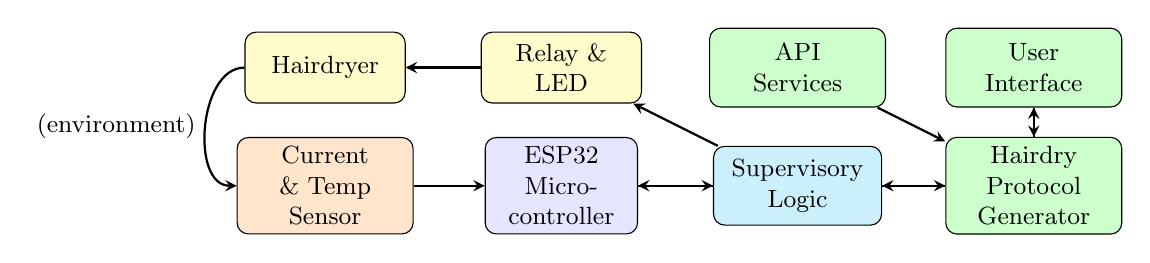
\begin{tikzpicture}[
    node distance=2cm and 2.5cm,
    box/.style={rectangle, draw, fill=blue!10, text width=2cm, align=center, rounded corners, minimum height=0.9cm, font=\small},
    sensor/.style={rectangle, draw, fill=orange!20, text width=2cm, align=center, rounded corners, minimum height=0.9cm, font=\small},
    logic/.style={rectangle, draw, fill=cyan!20, text width=1.9cm, align=center, rounded corners, minimum height=1cm, font=\small},
    actuator/.style={rectangle, draw, fill=yellow!20, text width=1.8cm, align=center, rounded corners, minimum height=0.9cm, font=\small},
    api/.style={rectangle, draw, fill=green!20, text width=2cm, align=center, rounded corners, minimum height=1cm, font=\small},
    arrow/.style={->, >=stealth, thick}
  ]

    \node[sensor] (sensor) at (0,-1.5) {Current \& Temp\\Sensor};
    \node[box, text width=1.7cm] (esp) at (3,-1.5) {ESP32\\Micro-\\controller};
    \node[logic] (logic) at (6,-1.5) {Supervisory\\Logic};

    \node[actuator] (relayled) at (3,0) {Relay \&\\LED};
    \node[actuator] (hairdryer) at (0,0) {Hairdryer};

    \node[api] (proto) at (9,-1.5) {Hairdry\\Protocol\\Generator};
    \node[api] (ui) at (9,0) {User\\Interface};
    \node[api] (api) at (6,0) {API\\Services};

    \draw[arrow] (hairdryer) to[out=180, in=180]node[left, font=\small] {(environment)} (sensor);
    \draw[arrow] (sensor) -- (esp);
    \draw[arrow] (esp) -- (logic);
    \draw[arrow] (logic) -- (esp);
    \draw[arrow] (logic) -- (relayled);
    \draw[arrow] (relayled) -- (hairdryer);
    \draw[arrow] (logic) -- (proto);
    \draw[arrow] (proto) -- (logic);
    \draw[arrow] (proto) -- (ui);
    \draw[arrow] (ui) -- (proto);
    \draw[arrow] (api) -- (proto);
    \vspace{1em}
  \end{tikzpicture}
  \vspace{.5em}
  \caption{System workflow.}
  \label{fig:workflow}
\end{figure}

Sensor measurements are acquired by the ESP32 microcontroller and forwarded to a Python-based supervisory control logic for real-time evaluation.

The supervisory control logic acts as the central decision unit, comparing sensor data with dynamically generated safety protocols obtained from an external API. Based on this evaluation, control commands are issued to the relay and LED module to actuate the hair dryer.

The color coding highlights different system layers: blue blocks represent sensing and control logic, while yellow blocks denote the physical actuation layer and green
blocks represnet a separate user interface visualizes system status and recommendations without directly affecting hardware control.
% Optional but often helpful:
\subsection{Requirements \& Success Criteria}
% Define what “works” means: sampling rate, RMS stability, temp thresholds, relay/LED behavior, API refresh cadence
% ==================================================


\paragraph{Functional Requirements}
The system shall:
\begin{itemize}
  \item Measure electrical current and temperature in real time during hair dryer operation.
  \item Compute stable RMS current values suitable for safety monitoring.
  \item Adapt safety thresholds based on hair thickness and hair porosity.
  \item Automatically disconnect the hair dryer via a relay when predefined safety limits are exceeded.
  \item Retrieve and apply safety protocols dynamically from an external API.
  \item Provide real-time visualization of system status and energy-related information.
\end{itemize}


\paragraph{Success Criteria}
The project is considered successful if:
\begin{itemize}
  \item Unsafe operating conditions consistently result in timely disconnection of the hair dryer.
  \item Sensor measurements are stable and correctly reflected in both the control logic and user interface.
  \item The system operates reliably in both hardware-in-the-loop and simulation modes.
  \item Users receive clear and interpretable feedback regarding energy usage and safety behavior.
\end{itemize}

\newpage
\section{Prototype Development --- Hardware}

\subsection{Load of Choice}
% Hair dryer: rated power, modes, expected current range, safety considerations, measurement approach

\noindent The \emph{Xiaomi High-speed Ionic Hair Dryer} Model GSHGL01LX is used as the primary electrical load. With a rated power of 1600 W at a mains voltage of 220–240 V, it is suitable for validating our sensing and control system in a household context. It is also commonplace, as one of the team members already owned the unit, simplifying setup and data collection. Specifics: \begin{itemize}
    \item A high-speed internal motor is used for efficient airflow and drying, reflecting typical household power consumption patterns of motorized heaters.
    \item The nominal electrical characteristics—220–240 V~ at up to 1600 W—yield a current draw of approximately 7 A at rated conditions, which is a useful range for testing the robustness of our current transformer and ADC interface.
    \item Using a real shunt load like a hair dryer adds practical relevance to the project compared to purely resistive or artificial loads, and allows us to observe non-idealities such as inrush currents and thermal effects that occur during typical usage.
    \item The device includes a detachable nozzle, making it a relevant choice for evaluating non-invasive current sensing and thermal monitoring for the prototype by inserting the sensors between the nozzle and the main outlet.
\end{itemize}

\begin{table}[H]
  \hfill
  \centering
  \begin{minipage}[t]{0.7\textwidth}
    \centering
    \caption{Specifications of the Hair Dryer (Xiaomi GSHGL01LX)~\cite{xiaomi_hairdryer_specs}.}
    \label{tab:hairdryer_specs}
    \begin{tabular}{ll}
      \toprule
      Attribute & Value \\
      \midrule
      Model & GSHGL01LX \\
      Rated Voltage & 220--240 V~ \\ 
      Rated Frequency & 50--60 Hz \\ 
      Rated Power & 1600 W \\ 
      Product Dimensions & 128.6 × 70 × 231 mm (without nozzle) \\ 
      Power Cord Length & 1.7 m \\ 
      Net Weight & 406 g (without nozzle and cord) \\
      \bottomrule
    \end{tabular}
  \end{minipage}%
  \hfill
  \begin{minipage}[t]{0.2\textwidth}
    \centering
    \captionof{figure}{Actual product.}
    \label{fig:hairdryer_image}
    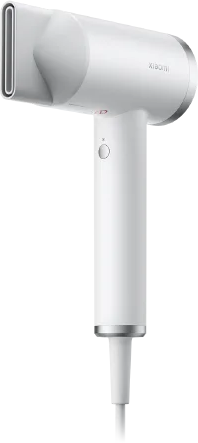
\includegraphics[width=0.6\linewidth]{figures/Xiaomi High-speed Ionic Hair Dryer.png}
  \end{minipage}
  \hfill
  \vspace{1em}
\end{table}


\subsection{Electronics}


\noindent Figure~\ref{fig:hardware_schematic} on the next page shows a schematic of the electronics of the prototype. The design integrates the mains-powered hairdryer with low-voltage sensing and control electronics, while maintaining isolation between high-voltage and low-voltage domains.

\paragraph{}Specifically, the hair dryer is connected to the AC mains, passing through an analog current transformer (SCT013) for real-time, non-invasive current measurement. The sensor output is conditioned, then digitized using an analog-to-digital converter (ADS1115), which communicates with a microcontroller (FireBeetle ESP32) via an I\textsuperscript{2}C bus. A temperature sensor module (LM35) is placed near the air outlet of the hair dryer, also connected to the microcontroller. A computer (not shown) handles control logic during testing to avoid reprogramming the microcontroller, which manages sensing and actuating. Control logic is not integrated for this prototype. All low-voltage components are powered from regulated DC supplies and share a common ground, while the AC side remains physically and electrically isolated for safety.


\begin{figure}[H]
  \centering
  
\includegraphics[width=.6\linewidth]{figures/ACEE_HardwareSchematic.pdf}
  \caption{Hardware schematic of the prototype.}
  \label{fig:hardware_schematic}
\end{figure}


% Table of parts: ESP32 FireBeetle, SCT013, ADS1115, DS18B20, relay/LED, resistors, wiring, enclosure, etc.
\begin{table}[H]
  \centering
  \begin{tabular}{lll}
    \toprule
    Component & Model & Purpose \\
    \midrule
    Microcontroller & ESP32 FireBeetle & Control + connectivity \\
    I/O expansion shield & Gravity & Wiring simplification \\
    ADC module (16-bit) & ADS1115 & High-resolution sampling \\
    Current sensor & SCT013 & Non-invasive AC current sensing \\
    Temperature sensor module & LM35 (DFR0023) & Outlet air temperature \\
    Digital relay module & HF3FA (DFR0473) &  Actuator: power cutoff \\
    LED module & DFR0021-B & Actuator: user feedback \\
    
    \bottomrule
  \end{tabular}
  \caption{Bill of materials.}
\end{table}

\begin{figure}[H]
\centering    
    % Row 1
    \begin{subfigure}[t]{0.3\textwidth}
        \centering
        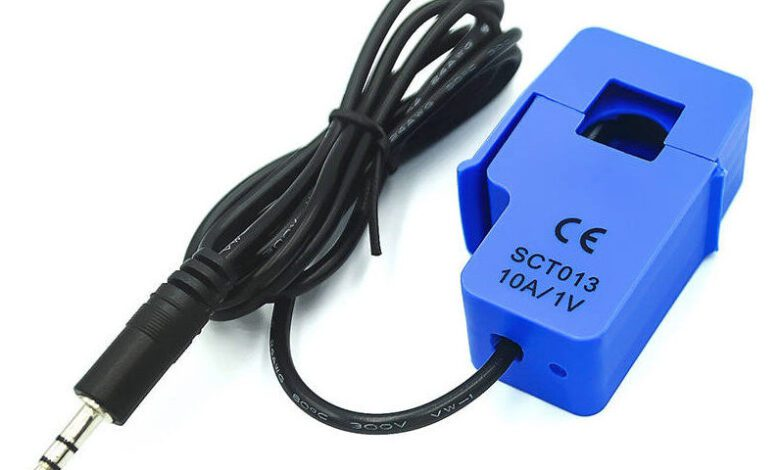
\includegraphics[height=2.4cm, keepaspectratio]{figures/SCT013_CurrentSensor.jpeg}
        \caption{SCT013 Current Sensor~\cite{yhdc_sct013}}
        \label{fig:SCT013}
    \end{subfigure}
    \hfill
    \begin{subfigure}[t]{0.3\textwidth}
        \centering
        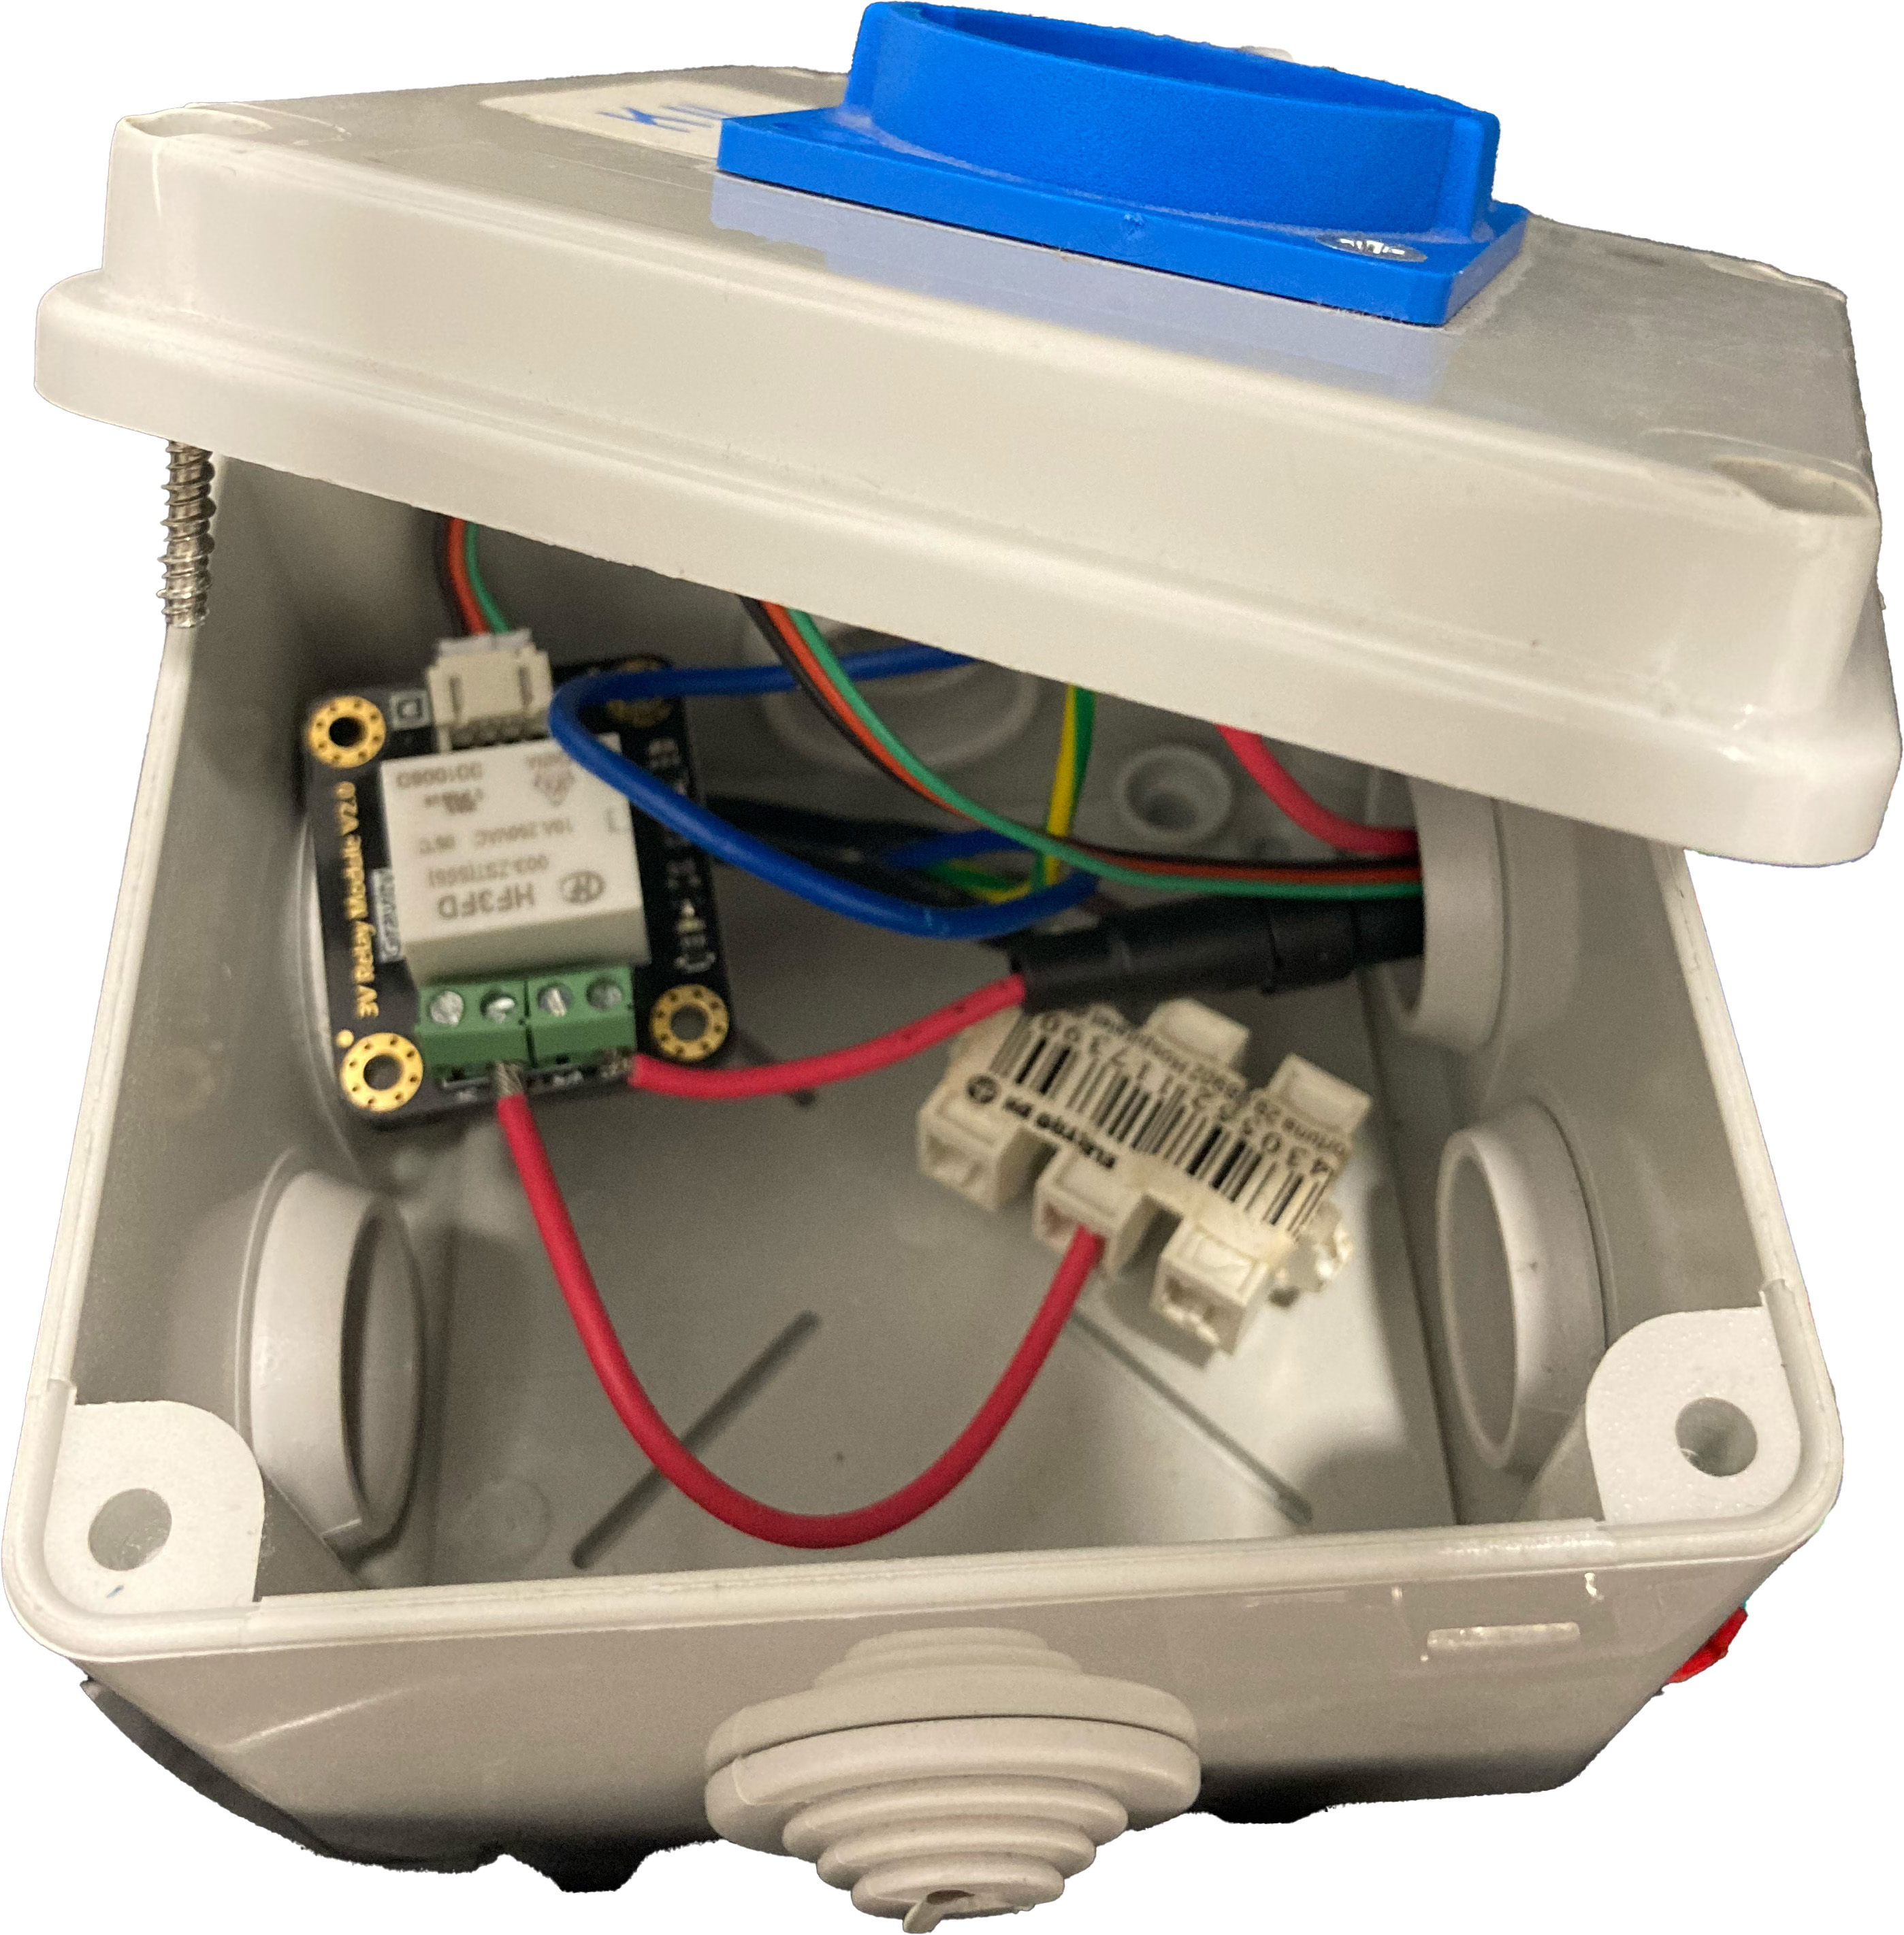
\includegraphics[height=2.4cm, keepaspectratio]{figures/ABB_SocketBox.jpg}
        \caption{Socket box with fuse and the relay in (c)}
        \label{fig:SocketBox}
    \end{subfigure}
    \hfill
    \begin{subfigure}[t]{0.3\textwidth}
        \centering
        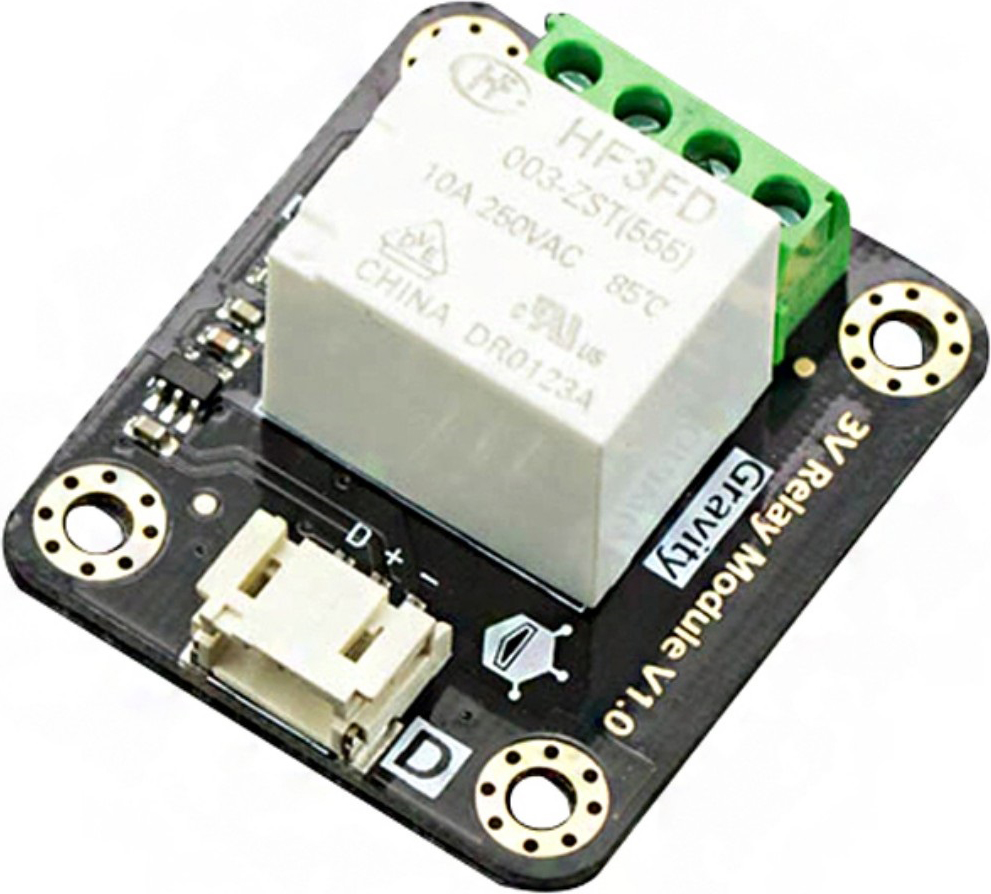
\includegraphics[height=2.4cm, keepaspectratio]{figures/GravityDigital10A_Relay.jpg}
        \caption{HF3FA Relay~\cite{dfrobot_relay_module_dfr0473}}
        \label{fig:HF3FD}
    \end{subfigure}
    
    % Row 2
    \begin{subfigure}[t]{0.3\textwidth}
        \centering
        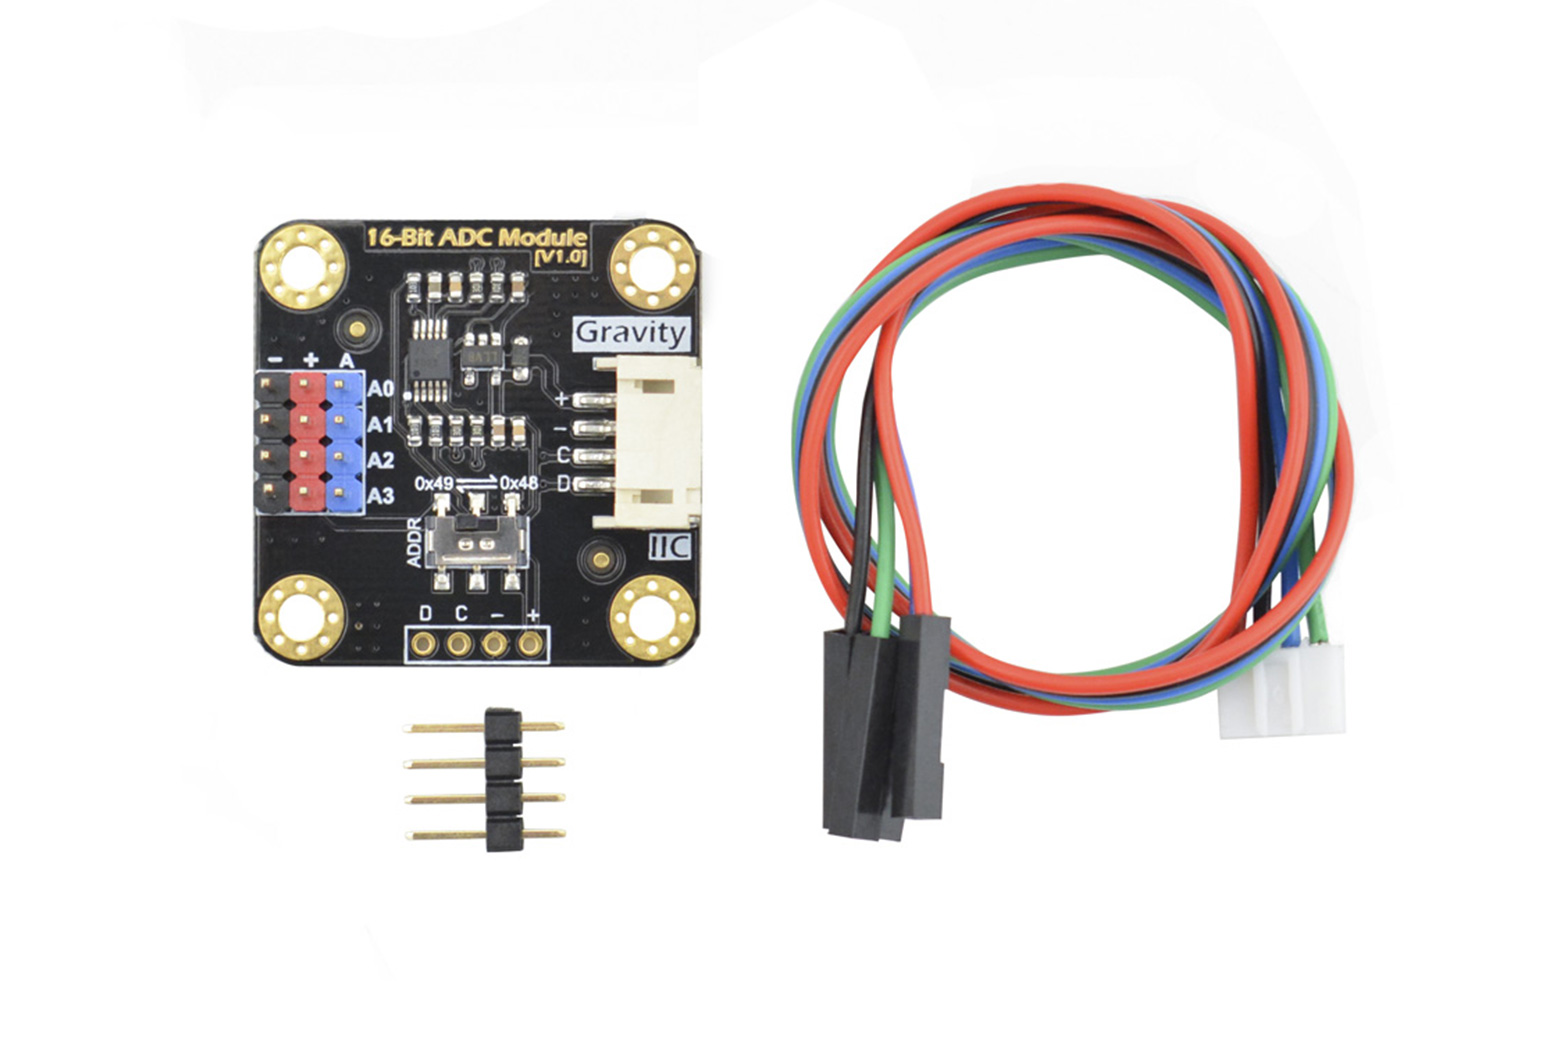
\includegraphics[height=2.4cm, keepaspectratio]{figures/ADS1115_16bitADCModule.jpg}
        \caption{ADS1115 ADC~\cite{ti_ads1115}}
        \label{fig:ADS1115}
    \end{subfigure}
    \hfill
    \begin{subfigure}[t]{0.3\textwidth}
        \centering
        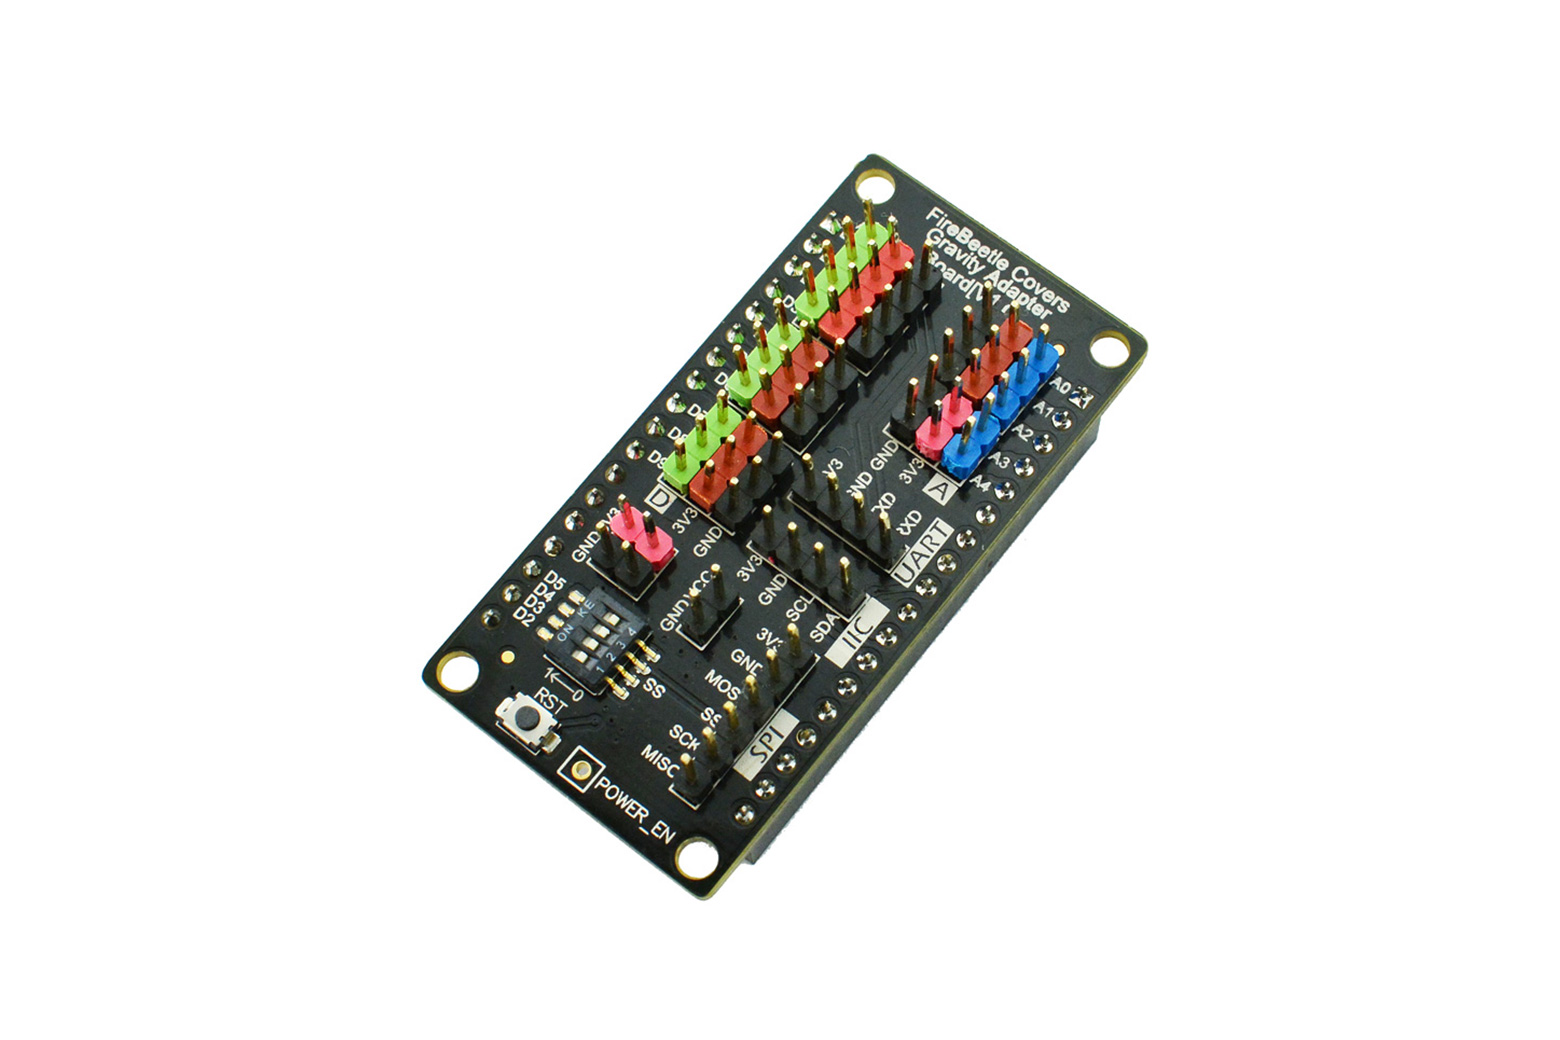
\includegraphics[height=2.4cm, keepaspectratio]{figures/GravityIOExpansionShield_FirebeetleCovers.jpg}
        \caption{I/O Expansion Shield~\cite{dfrobot_gravity_shield}}
        \label{fig:GravityShield}
    \end{subfigure}
    \hfill
    \begin{subfigure}[t]{0.3\textwidth}
        \centering
        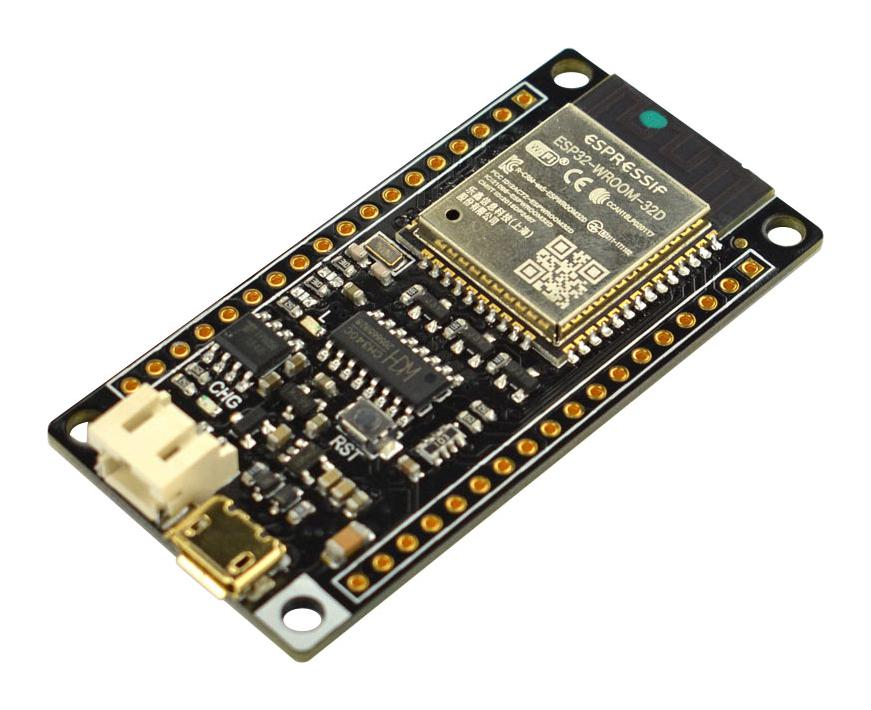
\includegraphics[height=2.4cm, keepaspectratio]{figures/ESP32_Microcontroller.jpg}
        \caption{FireBeetle ESP32~\cite{dfrobot_firebeetle_esp32}}
        \label{fig:ESP32}
    \end{subfigure}
    
    % Row 3
    \hfill
    \begin{subfigure}[t]{0.3\textwidth}
        \centering
        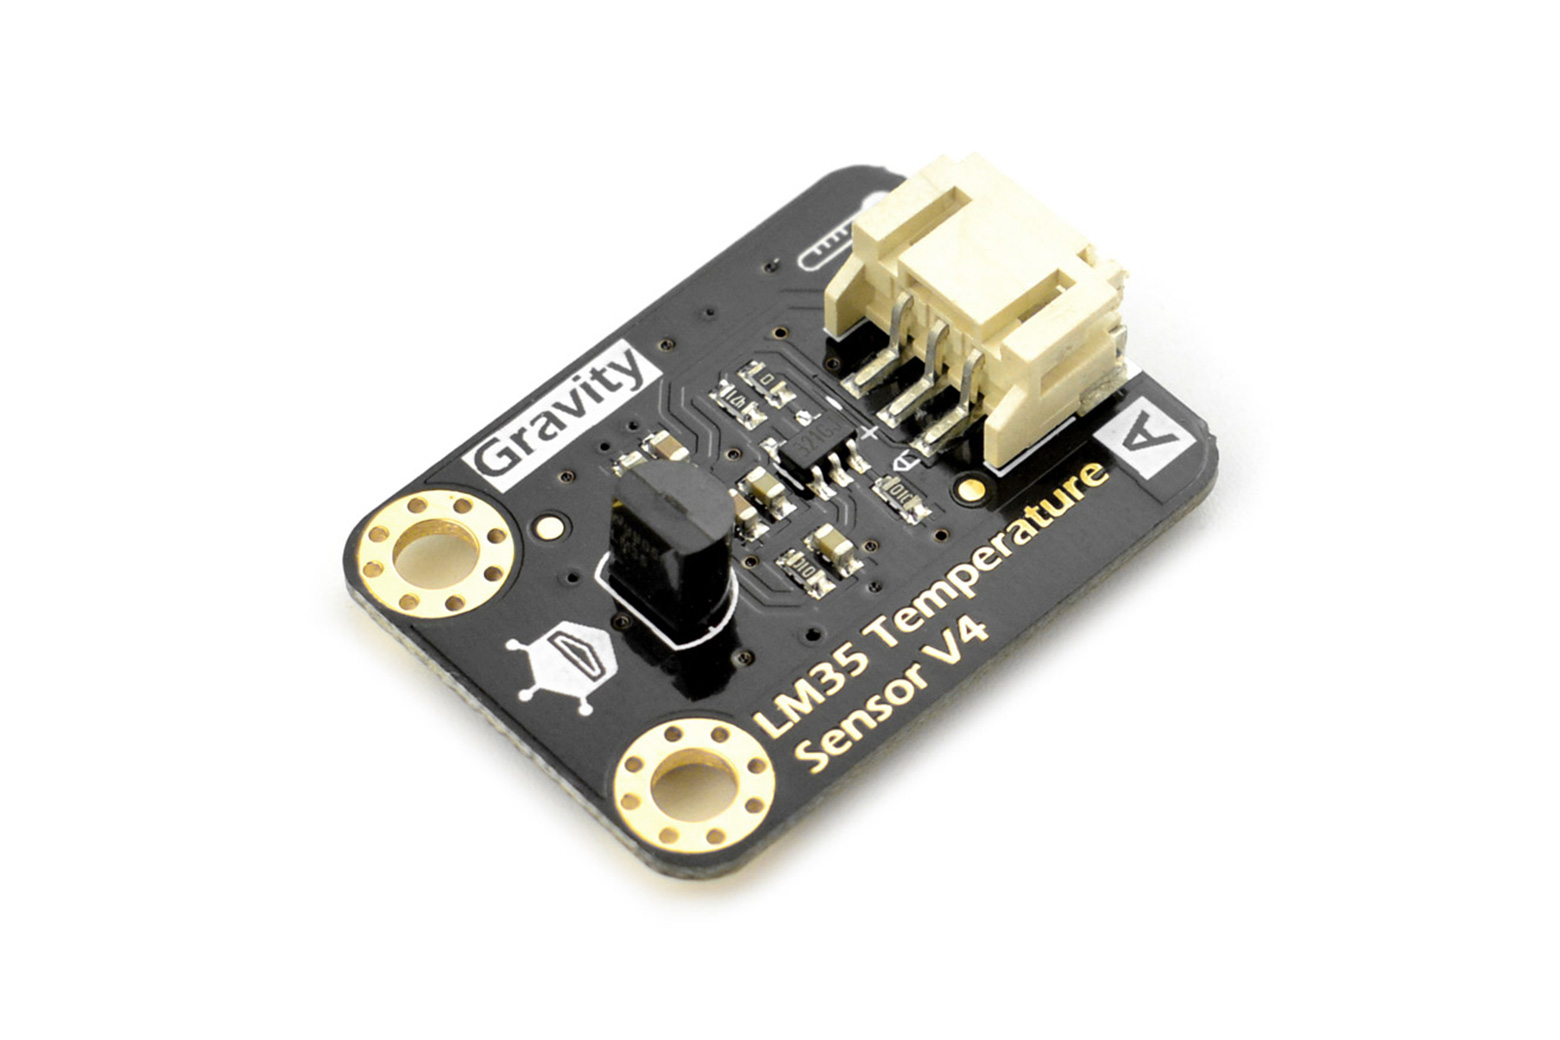
\includegraphics[height=2.4cm, keepaspectratio]{figures/LM35_TemperatureSensor.jpg}
        \caption{LM35 Sensor~\cite{lm35}}
        \label{fig:LM35}
    \end{subfigure}
    \hfill
    \begin{subfigure}[t]{0.3\textwidth}
        \centering
        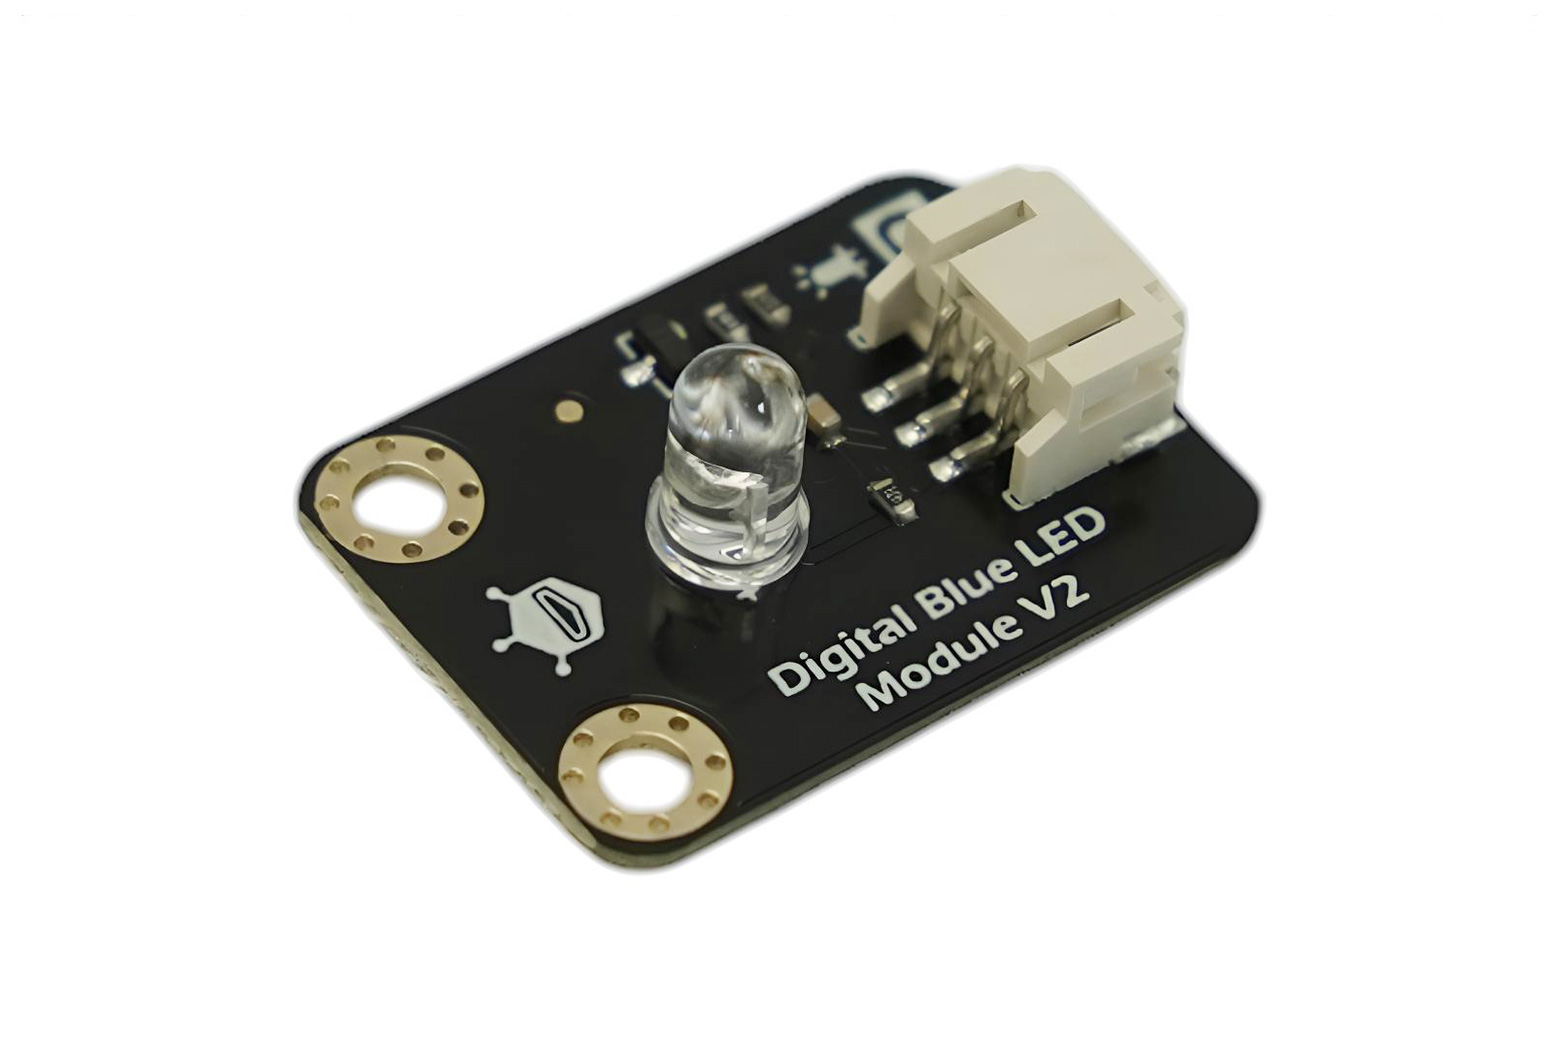
\includegraphics[height=2.4cm, keepaspectratio]{figures/BlueLED.jpg}
        \caption{Blue LED Module~\cite{dfrobot_led_module_dfr0021}}
        \label{fig:LED}
    \end{subfigure}
    \hfill
    \vspace{.5em}
    \caption{Hardware components used in the experimental setup.}
    \label{fig:hardware_components}
\end{figure}


\subsubsection*{Current Measurement Chain (SCT013 + Bias + ADS1115)}

The load current is measured using a non-invasive SCT013 current transformer, enabling galvanic isolation between the mains-powered appliance and the low-voltage measurement electronics. The sensor is clamped around the live conductor supplying the hair dryer, producing a secondary AC current proportional to the primary load current without requiring direct electrical contact.

The secondary output of the SCT013 is converted into a measurable voltage using a burden resistor, after which the signal is conditioned to interface with single-supply digital electronics. Since the sensor output is an AC waveform centered around 0\,V, a midpoint bias network referenced to half of the 3.3\,V supply is applied (1.65\,V). This bias shifts the waveform into the valid input range of the analog-to-digital converter while preserving its amplitude and phase information. Basic passive filtering is included to reduce high-frequency noise and improve signal stability.

The conditioned and biased voltage signal is digitized using an external ADS1115 16-bit analog-to-digital converter. The ADS1115 is configured for single-ended input operation and samples the current measurement signal on channel AIN1 with respect to ground. Compared to the ESP32’s internal ADC, the external ADC provides improved resolution, reduced noise sensitivity, and more repeatable measurements, which is particularly beneficial for low-frequency AC current monitoring.

All components of the current measurement chain operate in the low-voltage domain and share a common ground reference, while the SCT013 ensures electrical isolation from the high-voltage AC circuitry. This architecture allows safe and accurate acquisition of load current data suitable for further processing in software.

\subsubsection*{Temperature Measurement Chain (LM35)}

The outlet air temperature is measured using an LM35 analog temperature sensor, which provides an output voltage linearly proportional to temperature (10\,mV/\textdegree C). The sensor is powered from the 3.3\,V supply and referenced to the common low-voltage ground, ensuring compatibility with the ESP32 analog input range.

The LM35 output is connected directly to an ESP32 ADC input pin, as the sensor’s output voltage remains within safe limits for the microcontroller under the expected temperature range. Due to the analog nature of the signal, wiring between the sensor and the microcontroller was kept short to minimize noise pickup and ensure stable readings.

Physically, the sensor is positioned between the detachable nozzle and the main air outlet of the hairdryer, exposed to the outgoing airflow while avoiding direct contact with heating elements. This placement was determined through iteration: initial attempts to position the sensor outside the nozzle yielded readings that were too low to be useful for safety monitoring, as the airflow had already cooled significantly by that point. Moving the sensor to the position between the nozzle and the main outlet provides a representative measurement of operating temperature with acceptable response time, while reducing thermal stress and measurement instability caused by localized hot spots.

Basic validation of the temperature measurement was performed by comparing sensor output against ambient room temperature under no-load conditions and observing expected temperature rises during normal device operation. These checks confirmed correct sensor orientation, electrical connection, and thermal coupling prior to integration with the control logic.

\begin{figure}[H]
  \centering
  % 
\includegraphics[width=0.8\linewidth]{figures/LM35_TemperatureChain_Schematic}
  \caption{Close-up schematic of the LM35 temperature measurement chain and ESP32 ADC connection.}
  \label{fig:lm35_chain}
\end{figure}

\subsubsection*{Actuation Hardware (Blue LED / Relay Cutoff)}

System actuation and user feedback are provided through a low-voltage relay and a blue status LED module, both controlled by the ESP32 via digital GPIO pins. The relay enables electrical isolation between the low-voltage control electronics and the mains-powered load, allowing the system to enable or disable the appliance safely.

The relay control input is driven by a dedicated GPIO pin configured as a digital output. The relay module incorporates the required driver and isolation circuitry to interface directly with 3.3\,V logic levels, ensuring reliable switching while preventing high-voltage transients from propagating to the microcontroller. The relay contacts are located exclusively on the mains side of the circuit.

Visual system feedback is provided by a DFRobot digital blue LED module connected to a separate GPIO pin. The module integrates the LED and its current-limiting circuitry on-board, allowing it to be driven directly from a 3.3\,V digital output without the need for an external series resistor. This simplifies wiring and reduces component count while maintaining safe operating conditions. The LED operates entirely within the low-voltage domain and provides a clear indication of system state (e.g., relay enabled or disabled).

\begin{figure}[H]
  \centering
  % 
\includegraphics[width=0.6\linewidth]{figures/Actuation_LED_Relay_Schematic.pdf}
  \caption{Close-up schematic of the relay cutoff and blue LED module actuation circuitry controlled by the ESP32.}
  \label{fig:actuation_chain}
\end{figure}


\subsection{Hardware Build Photos}
\begin{figure}[H]
  \centering
  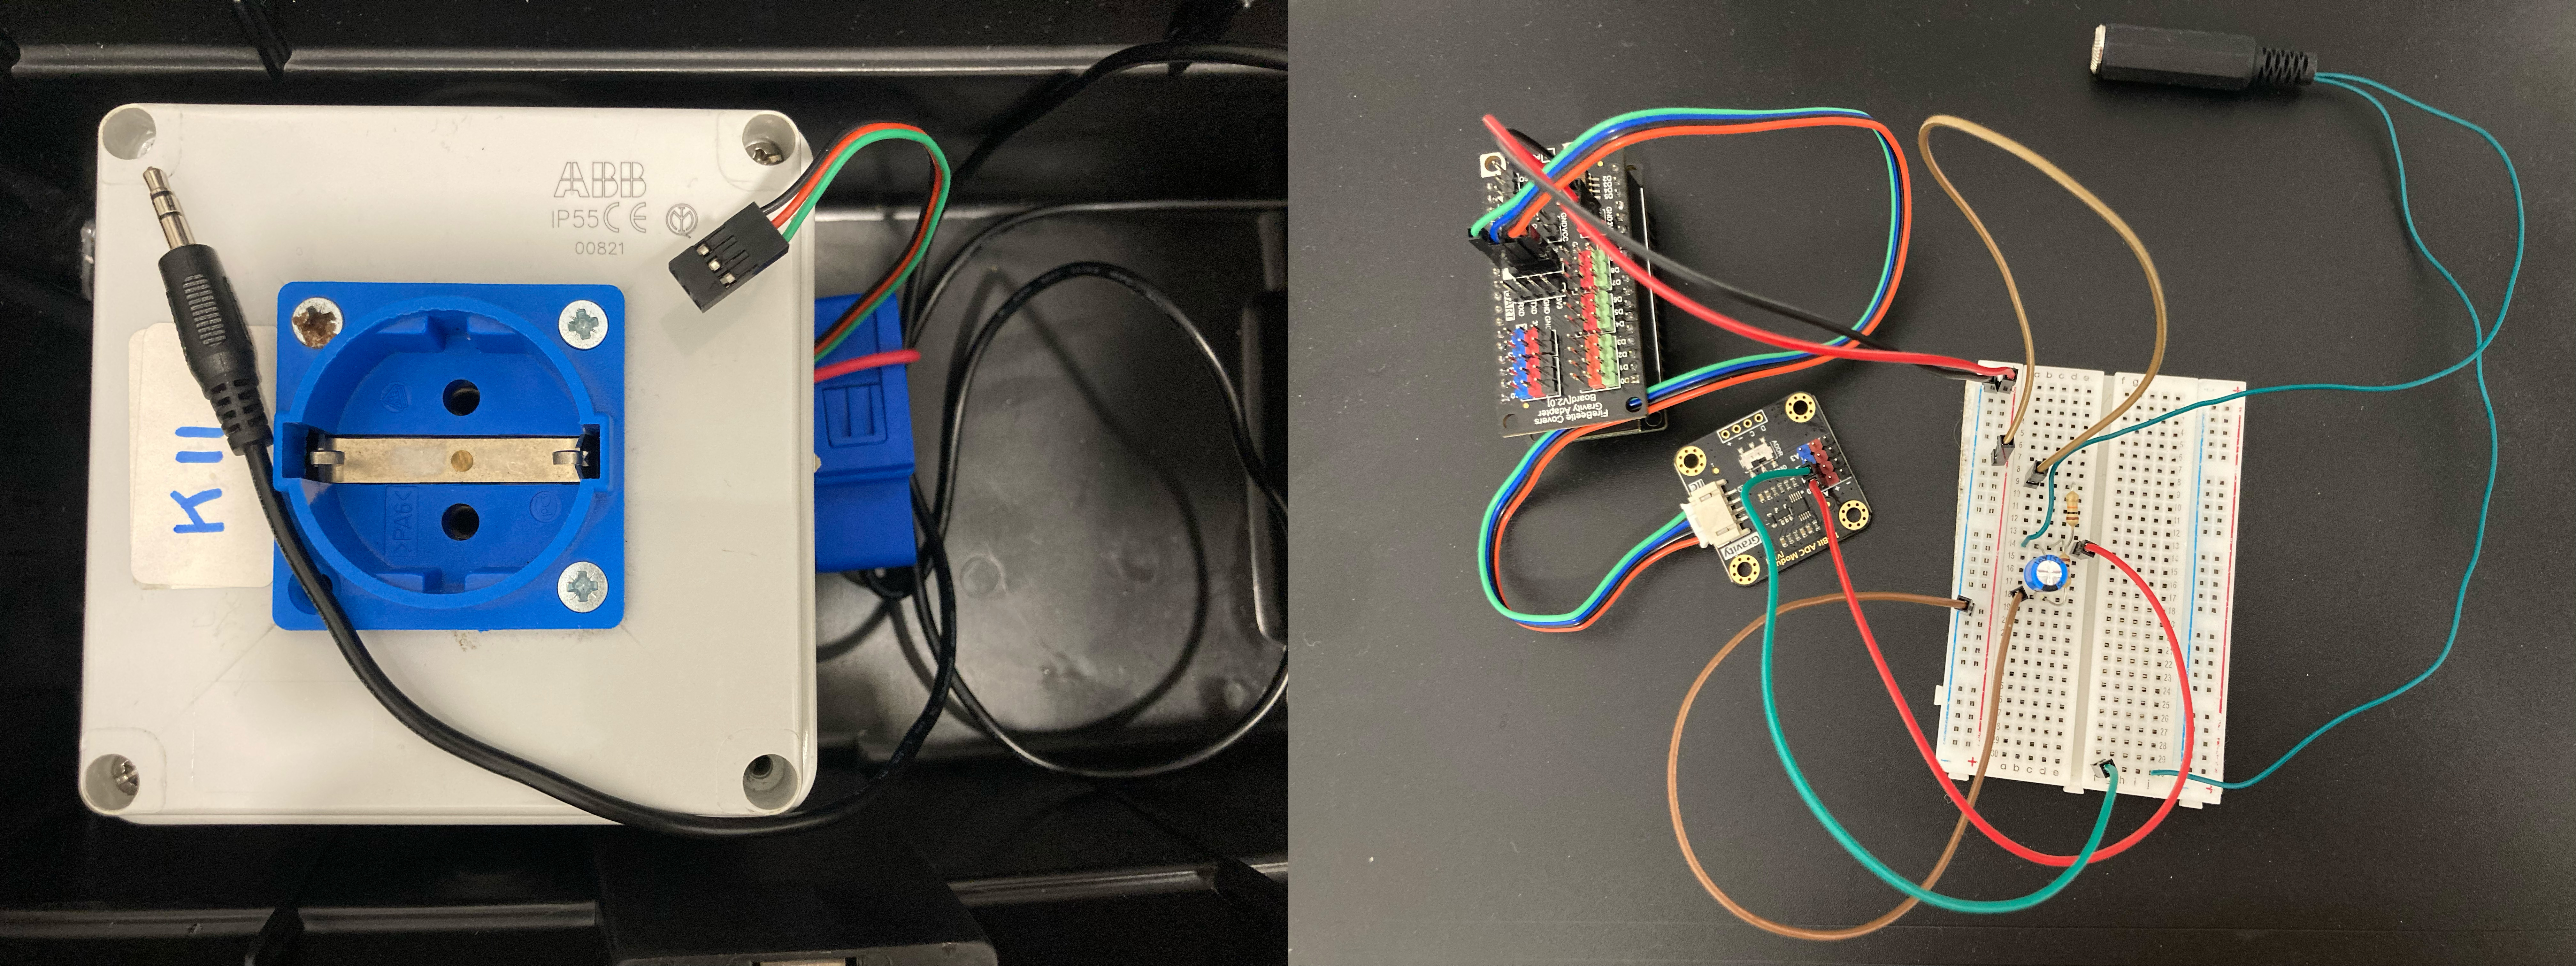
\includegraphics[width=0.6\linewidth]{figures/IMG_6610.jpg}
  \caption{Hardware: AC side and DC side.}
\end{figure}
\begin{figure}[H]
  \centering
  %\includegraphics[width=0.85\linewidth]{figures/.jpg}
  \caption{Hardware: full setup.}
\end{figure}

% ==================================================
\newpage
\section{Prototype Development --- Software}

\begin{figure}[H]
  \centering
  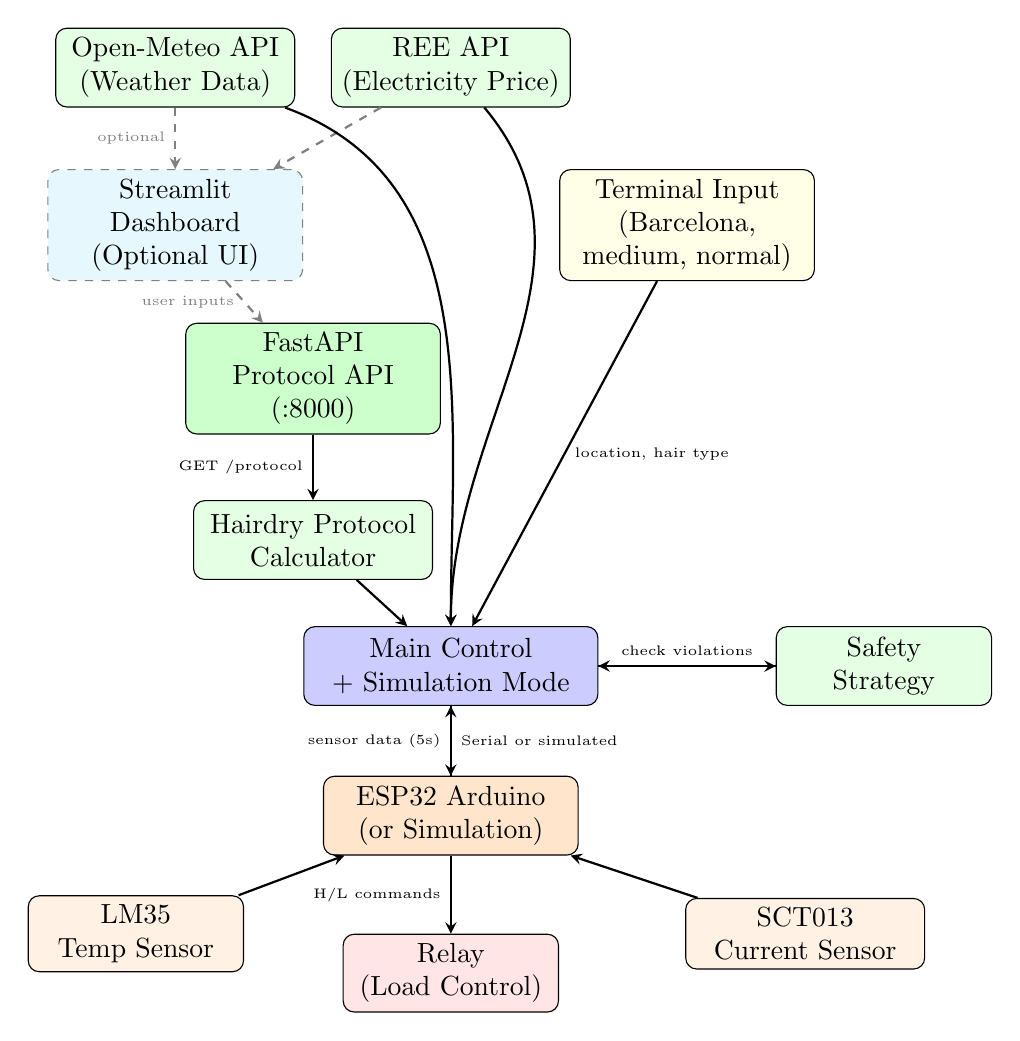
\begin{tikzpicture}[
    node distance=1.5cm and 2cm,
    box/.style={rectangle, draw, fill=blue!10, text width=3cm, align=center, rounded corners, minimum height=1cm},
    api/.style={rectangle, draw, fill=green!10, text width=2.8cm, align=center, rounded corners, minimum height=1cm},
    sensor/.style={rectangle, draw, fill=orange!10, text width=2.5cm, align=center, rounded corners, minimum height=0.8cm},
    arrow/.style={->, >=stealth, thick},
    dashed_arrow/.style={->, >=stealth, thick, dashed, gray}
  ]

    % Top layer - External APIs
    \node[api] (openmeteo) at (-1.5,0) {Open-Meteo API\\(Weather Data)};
    \node[api] (ree) at (2,0) {REE API\\(Electricity Price)};

    % Second layer - Dashboard (OPTIONAL)
    \node[box, fill=cyan!10, dashed, draw=gray] (dashboard) at (-1.5,-2) {Streamlit\\Dashboard\\(Optional UI)};

    % Terminal Input (Alternative to Dashboard)
    \node[box, fill=yellow!10] (terminal) at (5,-2) {Terminal Input\\(Barcelona, medium, normal)};

    % Third layer - API Layer
    \node[box, fill=green!20] (fastapi) at (0.25,-3.95) {FastAPI\\Protocol API\\(:8000)};

    % Fourth layer - Calculation Module
    \node[api] (calculator) at (0.25,-6) {Hairdry Protocol\\Calculator};

    % Fifth layer - Main Control
    \node[box, fill=blue!20, text width=3.5cm] (mainpy) at (2,-7.6) {Main Control\\+ Simulation Mode};

    % Sixth layer - Safety Strategy
    \node[api, text width=2.5cm] (safety) at (7.5,-7.6) {Safety\\Strategy};

    % Bottom layer - Arduino (or Simulation)
    \node[box, fill=orange!20] (arduino) at (2,-9.5) {ESP32 Arduino\\(or Simulation)};

    % Sensors
    \node[sensor] (temp) at (-2,-11) {LM35\\Temp Sensor};
    \node[sensor, text width=2.8cm] (current) at (6.5,-11) {SCT013\\Current Sensor};

    % Actuator
    \node[sensor, fill=red!10] (relay) at (2,-11.5) {Relay\\(Load Control)};

    % Arrows - Data flow
    \draw[dashed_arrow] (openmeteo) -- node[left, font=\tiny, text=gray] {optional} (dashboard);
    \draw[dashed_arrow] (ree) -- (dashboard);
    \draw[arrow] (openmeteo) to[out=-20, in=90] (mainpy);
    \draw[arrow] (ree) to[out=-50, in=90] (mainpy);
    \draw[dashed_arrow] (dashboard) -- node[left, font=\tiny, text=gray] {user inputs} (fastapi);
    \draw[arrow] (terminal) -- node[right, font=\tiny] {location, hair type} (mainpy);
    \draw[arrow] (fastapi) -- node[left, font=\tiny] {GET /protocol} (calculator);
    \draw[arrow] (calculator) -- (mainpy);
    \draw[arrow] (mainpy) -- node[above, font=\tiny] {check violations} (safety);
    \draw[arrow] (safety) -- (mainpy);
    \draw[arrow] (mainpy) -- node[right, font=\tiny] {Serial or simulated} (arduino);
    \draw[arrow] (arduino) -- node[left, font=\tiny] {sensor data (5s)} (mainpy);
    \draw[arrow] (temp) -- (arduino);
    \draw[arrow] (current) -- (arduino);
    \draw[arrow] (arduino) -- node[left, font=\tiny] {H/L commands} (relay);

  \end{tikzpicture}
  \caption{Software schematic showing dual operation modes: standalone terminal-based control (solid lines) with direct API access and default values, or optional dashboard interface (dashed lines). Simulation mode enables hardware-free software testing.}
  \label{fig:software_schematic}
\end{figure}

\subsection{Software Architecture}

The software system operates in two distinct modes with six primary modules in a distributed architecture:

\textbf{Operation Modes:} The system supports both \emph{standalone terminal mode} (default) and \emph{dashboard-assisted mode}. In standalone mode, executed via \texttt{run\_integrated.bat} or direct Python invocation, users provide inputs through terminal prompts (location, hair type, porosity), and the main control system directly fetches weather and electricity data from external APIs with built-in fallback values (Barcelona, medium hair, normal porosity). In dashboard mode, launched via \texttt{run.bat}, a Streamlit web interface provides graphical input and visualization while the same backend services handle protocol generation and safety monitoring. Both modes share identical protocol calculation and safety enforcement logic, differing only in user interface presentation.

\textbf{ESP32 Arduino Firmware} (\texttt{Integrated\_Project.ino}) implements the lowest-level hardware interface, reading analog sensors through an ADS1115 16-bit ADC for current measurement and the ESP32's built-in ADC for temperature. The firmware samples current at 1 kHz to calculate RMS values over 20 ms intervals, then averages 250 RMS samples to produce one filtered output every 5 seconds. It communicates via serial at 115200 baud, responding to relay control commands (`H' for high/on, `L' for low/off) and transmitting sensor readings in the format: \texttt{Temperature: XX.XX | Current: X.XXXXX}.

\textbf{Main Control System} (\texttt{Integrated\_Project.py}) serves as the central coordinator, managing three key responsibilities:
\begin{itemize}[leftmargin=*]
  \item Serial communication with the ESP32 through the \texttt{SerialBoard} class
  \item Protocol acquisition from the local API with user-specific parameters
  \item Real-time safety monitoring by feeding sensor data to the \texttt{SafetyStrategy} module
\end{itemize}
It runs a continuous monitoring loop synchronized to the Arduino's 5-second output interval, checking for threshold violations and commanding relay shutdown when safety limits are exceeded. This module implements \emph{simulation mode}: when Arduino connection fails, it generates synthetic sensor data (temperature ramping 65-89°C, current cycling 5-7 A) with realistic 5-second timing, enabling complete software testing without physical hardware. The simulation follows the same code paths as real operation, validating protocol logic, safety enforcement, and user interaction flows.

\textbf{Protocol API} (\texttt{mock\_protocol\_api.py}) provides a RESTful interface via FastAPI at port 8000, accepting query parameters including room temperature, humidity, hair type, porosity, towel-dry level, time priority, and safety thresholds. It delegates calculation logic to the protocol calculator module and returns a JSON response specifying sensor-specific thresholds (temperature and current) with corresponding duration limits.

\textbf{Protocol Calculator} (\texttt{protocol\_calculator.py}) implements the core recommendation engine, calculating optimal drying parameters based on environmental factors and user characteristics. It computes a drying power index from temperature and humidity, determines appropriate heat settings (Low/Medium/High), estimates bulk and finish phase durations, and generates safety protocol thresholds. It also interfaces with external APIs to fetch real-time room conditions from Open-Meteo and electricity prices from the Spanish REE API or regional fallback values.

\textbf{Safety Strategy Module} (\texttt{safety\_strategy.py}) monitors sensor readings against protocol thresholds with duration-based violation detection. For each condition (temperature and current), it starts a timer when thresholds are exceeded and triggers shutdown if conditions persist. It implements hysteresis by resetting timers when values normalize, preventing false triggers.

\textbf{Streamlit Dashboard} (\texttt{StreamlitDashboard.py}) provides a web-based user interface for inputting location, hair characteristics (type and porosity), and viewing personalized drying protocols. It displays environmental conditions, recommended drying phases (towel-dry, optional air-dry, bulk heat, and finish), total time estimates, and energy cost analysis across multiple time-priority and towel-dry level combinations. The dashboard visualizes cost trade-offs through interactive charts, helping users select optimal drying strategies.

\subsection{Data Streams and Sources}

The system integrates multiple external and internal data sources with specific update frequencies and failure handling:

\textbf{Open-Meteo Weather API} provides current temperature and relative humidity for specified locations. Two endpoints are used: geocoding API converts location names to coordinates, and forecast API returns weather data with temperature and humidity fields. Both dashboard and main control system access this API, enabling standalone operation. Requests timeout after 5 seconds with fallback to Barcelona coordinates or default values (20°C, 60\% humidity) on failure.

\textbf{REE Electricity Price API} delivers Spanish real-time electricity prices with hourly granularity. The system queries current hour's price in €/MWh and converts to €/kWh. Both UI modes access this via unified function. For non-Spanish locations or API failures, a regional price map provides fallback values ranging from 0.14 to 0.35 €/kWh.

\textbf{Arduino Sensor Data Stream} transmits temperature and current readings every 5 seconds over serial. Temperature measurements use the LM35's linear 10 mV/°C characteristic: $T = V \times 100$, where $V$ is the ADC voltage. Current measurements undergo two-stage filtering: RMS calculation over 20 ms windows (matching AC power frequency), then averaging 250 RMS samples for noise reduction. The 5-second interval balances responsiveness with computational efficiency, as the ESP32 performs $250 \times 20 = 5000$ ms of RMS integration per output. In \emph{simulation mode} (triggered when \texttt{SerialBoard.connect()} fails), the main control system generates synthetic sensor data matching the same timing and format: temperature values cycle from 65°C to 89°C with random noise ($\pm 1^\circ C$), and current cycles from 5.0 to 7.0 A with noise ($\pm 0.1$ A). This simulation maintains the 5-second update cadence and identical data format (\texttt{Temperature: XX.XX | Current: X.XXXXX}), enabling full protocol validation, threshold testing, and UI verification without physical hardware.

\textbf{Serial Communication Protocol} uses a simple ASCII format for bidirectional communication at 115200 baud. Commands from Python to Arduino consist of single characters (`H' for relay on, `L' for relay off, `PING' for handshake verification). Sensor data from Arduino follows the template \texttt{Temperature: XX.XX | Current: X.XXXXX}, parsed by splitting on the pipe character and extracting float values after colons. The Python \texttt{SerialBoard} class buffers incoming data in a background thread, updating \texttt{latest\_temp} and \texttt{latest\_current} attributes that the main control loop reads.

\subsection{Control and Recommendation Logic}

The system implements three-tier safety thresholds with duration-based triggering and hysteresis:

\textbf{Temperature Threshold Monitoring:} The protocol specifies a maximum temperature (e.g., 38°C measured at sensor location) and total duration limit based on calculated drying time. When sensor temperature exceeds threshold, \texttt{SafetyStrategy} records the violation timestamp. If temperature remains elevated for the full duration (e.g., total drying time of 4.2 minutes = 252 seconds in demo mode), the system triggers shutdown with the message "You used too long the total hairdrying duration." If temperature drops below threshold before duration expires, the timer resets, implementing hysteresis to prevent oscillation.

\textbf{Current Threshold Monitoring:} High current indicates high heat mode usage on the hairdryer. The system monitors for sustained current above threshold (e.g., 5.0 A) for the bulk phase duration (e.g., 2.4 minutes). This prevents prolonged high-heat exposure that could damage hair, triggering shutdown with "You used too long the high heat mode in your hairdryer" when violated. The duration corresponds to the bulk drying phase, allowing sufficient time for the high-heat portion while preventing overuse.

\textbf{Maximum Runtime Limit:} A failsafe 30-minute (1,800,000 ms) absolute runtime limit prevents indefinite operation regardless of sensor readings. This protects against sensor failures or unexpected usage patterns. In demo mode, all durations divide by 10 for faster testing (e.g., 30 minutes becomes 3 minutes).

\textbf{Hysteresis Implementation:} The \texttt{SafetyStrategy.check\_violations()} method maintains per-condition state including \texttt{triggered\_at} timestamps. Violations only count when continuously exceeding thresholds for full durations. Dropping below threshold at any point resets the timer to \texttt{None}, requiring a fresh sustained violation to trigger shutdown. This design prevents false alarms from brief temperature spikes or momentary high-heat bursts during normal hair manipulation.

\textbf{Recommendation Engine:} The protocol calculator determines heat settings through a multi-factor index. Starting with a hair-type baseline (fine=0, medium=1, thick=2), it adjusts for porosity (low +1, high -1), environmental drying power (DP $< 0.6$ adds +1, DP $> 1.2$ subtracts -1), and time priority (scaled by $0.5 \times (\text{priority} - 0.5)$). The final heat index, clamped to 0-2, maps to Low (50-60°C), Medium (70-80°C), or High (90-100°C) settings.

Drying time calculation begins with a base bulk time:
\begin{equation}
t_{\text{bulk}} = \left(2 + \frac{\text{towel\_level} - 50}{25}\right) \times k_{\text{hair}} \div \left(0.5 + 0.5 \times \text{DP}\right) \div \left(1 + 0.3 \times \text{priority}\right)
\end{equation}
where $k_{\text{hair}} = \{0.7, 1.0, 1.4\}$ for fine/medium/thick hair. The finish time follows a similar formula with different coefficients. For favorable conditions (temp $\geq 18$\textdegree C, humidity $< 75\%$, DP $\geq 0.5$, priority $\leq 0.7$), the system recommends hybrid drying: 10-30 minutes of air drying followed by reduced blow-dry times (bulk $\times 0.6$, finish $\times 0.7$).

\subsection{Details of Key Algorithms and Communications}

\textbf{RMS Current Calculation:} The firmware computes true RMS using numerical integration synchronized to the AC power frequency (50 Hz). For each 1 ms timestep:
\begin{equation}
S_{\text{RMS}} = S_{\text{RMS}} + i^2(t) \cdot \Delta t
\end{equation}
where $i(t) = (V_{\text{ADC}} - 1.65) \times 30$ converts the SCT013's AC-coupled voltage to current, and $\Delta t$ in seconds is tracked by the microcontroller. After accumulating 20 samples (20 ms = one AC period at 50 Hz):
\begin{equation}
I_{\text{RMS}} = \sqrt{f \cdot S_{\text{RMS}}}
\end{equation}
where $f = 50$ Hz. The factor of frequency converts the time-integrated sum to proper RMS. This method accurately captures non-sinusoidal waveforms from variable-speed hairdryer motors.

\textbf{Multi-Stage Filtering:} Raw RMS values undergo moving average filtering over 250 samples to reject high-frequency noise and short-term variations:
\begin{equation}
I_{\text{filtered}} = \frac{1}{250} \sum_{k=0}^{249} I_{\text{RMS}}[k]
\end{equation}
This 5-second averaging window (250 samples $\times$ 20 ms) provides stable readings while remaining responsive to actual usage changes. Values below 0.1 A are clamped to zero to eliminate sensor offset noise.

\textbf{Serial Communication Handshake:} On connection, the Python client sends a PING command and waits 500 ms for "OK" or "PONG" response. If no response arrives but the serial port opened successfully, the system assumes valid connection and proceeds. This allows operation even if the Arduino firmware doesn't implement PING, while providing verification when available.

\textbf{Automatic Port Discovery:} The \texttt{SerialBoard} class iterates through all available ports, attempting connection to each until successful. For each port, it opens the connection, waits 2 seconds for ESP32 initialization, attempts handshake, and moves to the next port on failure. This eliminates manual configuration.

\textbf{Threaded Sensor Reading:} A daemon thread runs \texttt{read\_sensor\_data()} continuously, parsing incoming serial lines and updating \texttt{latest\_temp} and \texttt{latest\_current} attributes. The main control loop reads these attributes every 5 seconds, decoupling sensor I/O from safety logic. Thread synchronization relies on Python's GIL, as float assignments are atomic operations.

\textbf{Demo Mode Acceleration:} Setting \texttt{DEMO\_MODE = 1} divides all protocol durations by 10 before sending to \texttt{SafetyStrategy}, allowing rapid testing (e.g., 4-minute protocols become 24 seconds). Critically, this only affects safety timeout durations, not the Arduino's sensor sampling or output rate, maintaining realistic sensor data flow during accelerated testing.

\textbf{Multi-Service Launcher Architecture:} The \texttt{run.bat} script orchestrates three independent services: FastAPI protocol server (port 8000), Streamlit dashboard (port 8501), and main control system with serial connection. Services launch sequentially with configurable delays to ensure dependencies initialize. The script supports optional ngrok tunneling via \texttt{--ngrok} for remote access, dynamically setting environment variables (\texttt{API\_URL}, \texttt{DASHBOARD\_URL}) that the control system reads. For standalone operation, \texttt{run\_integrated.bat} bypasses dashboard and API, launching only the main control script. This provides protocol data via local FastAPI or falls back to hardcoded defaults if unreachable.
\begin{figure}[H]
  \centering
  % \includegraphics[width=0.9\linewidth]{figures/dashboard.png}
  \caption{Example UI/logging screenshot.}
\end{figure}

% ==================================================
\newpage
\section{Testing and Validation Iterations}

\begin{figure}[H]
  \centering
  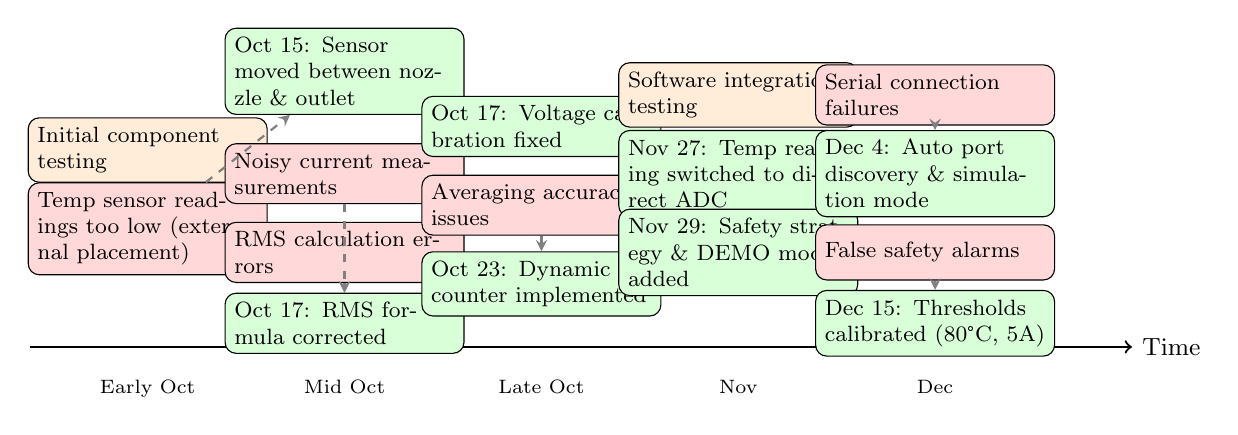
\begin{tikzpicture}[
    node distance=0.8cm,
    phase/.style={rectangle, draw, fill=blue!15, text width=2.8cm, align=left, rounded corners, minimum height=0.7cm, font=\footnotesize},
    issue/.style={rectangle, draw, fill=red!15, text width=2.8cm, align=left, rounded corners, minimum height=0.7cm, font=\footnotesize},
    fix/.style={rectangle, draw, fill=green!15, text width=2.8cm, align=left, rounded corners, minimum height=0.7cm, font=\footnotesize},
    test/.style={rectangle, draw, fill=orange!15, text width=2.8cm, align=left, rounded corners, minimum height=0.7cm, font=\footnotesize},
    arrow/.style={->, >=stealth, thick}
  ]
    % Timeline axis
    \draw[thick, ->] (0,0) -- (14,0) node[right, font=\small] {Time};

    % Month labels
    \node[below, font=\scriptsize] at (1.5,-0.3) {Early Oct};
    \node[below, font=\scriptsize] at (4,-0.3) {Mid Oct};
    \node[below, font=\scriptsize] at (6.5,-0.3) {Late Oct};
    \node[below, font=\scriptsize] at (9,-0.3) {Nov};
    \node[below, font=\scriptsize] at (11.5,-0.3) {Dec};

    % Events - staggered vertically for readability
    % Early October
    \node[test] (test1) at (1.5,2.5) {Initial component testing};
    \node[issue] (issue1) at (1.5,1.5) {Temp sensor readings too low (external placement)};

    % Mid October
    \node[fix] (fix1) at (4,3.5) {Oct 15: Sensor moved between nozzle \& outlet};
    \node[issue] (issue2) at (4,2.2) {Noisy current measurements};
    \node[issue] (issue3) at (4,1.2) {RMS calculation errors};
    \node[fix] (fix2) at (4,0.3) {Oct 17: RMS formula corrected};

    % Late October
    \node[fix] (fix3) at (6.5,2.8) {Oct 17: Voltage calibration fixed};
    \node[issue] (issue4) at (6.5,1.8) {Averaging accuracy issues};
    \node[fix] (fix4) at (6.5,0.8) {Oct 23: Dynamic counter implemented};

    % November
    \node[test] (test2) at (9,3.2) {Software integration testing};
    \node[fix] (fix5) at (9,2.2) {Nov 27: Temp reading switched to direct ADC};
    \node[fix] (fix6) at (9,1.2) {Nov 29: Safety strategy \& DEMO mode added};

    % December
    \node[issue] (issue5) at (11.5,3.2) {Serial connection failures};
    \node[fix] (fix7) at (11.5,2.2) {Dec 4: Auto port discovery \& simulation mode};
    \node[issue] (issue6) at (11.5,1.2) {False safety alarms};
    \node[fix] (fix8) at (11.5,0.3) {Dec 15: Thresholds calibrated (80°C, 5A)};

    % Connecting arrows (selected key paths)
    \draw[arrow, dashed, gray] (issue1) -- (fix1);
    \draw[arrow, dashed, gray] (issue2) -- (fix2);
    \draw[arrow, dashed, gray] (issue3) -- (fix2);
    \draw[arrow, dashed, gray] (issue4) -- (fix4);
    \draw[arrow, dashed, gray] (issue5) -- (fix7);
    \draw[arrow, dashed, gray] (issue6) -- (fix8);

  \end{tikzpicture}
  \caption{Timeline of testing activities, identified issues, and implemented mitigations during prototype development (October--December 2025).}
  \label{fig:testing_timeline}
\end{figure}

\subsection{Test Plan}

Testing was conducted incrementally, validating individual components before integration. No external test equipment was used beyond the prototype itself and standard development tools (serial monitor, Python scripts).

\subsubsection*{Component-Level Testing}

\paragraph{Current Sensor (SCT013)}
The current transformer was tested by connecting it to the hairdryer and observing readings at different power settings. Initial tests revealed noisy measurements, leading to implementation of two-stage filtering: 20 ms RMS calculation synchronized to AC frequency, followed by 250-sample moving average producing stable 5-second updates. Values below 0.1 A were clamped to zero to eliminate sensor offset noise.

\paragraph{Temperature Sensor (LM35)}
Temperature measurements were validated by comparing sensor output against ambient room temperature under no-load conditions. During hairdryer operation, the sensor was positioned near the air outlet to observe expected temperature rises. The linear relationship (10 mV/°C) was verified by checking voltage-to-temperature conversion in the ESP32 ADC range.

\paragraph{Relay and LED}
Actuation hardware was tested using simple serial commands (`H' for high, `L' for low) sent from the Python control script. The relay switching was audibly confirmed, and LED visual feedback verified proper GPIO control.

\paragraph{Serial Communication}
ESP32-to-Python communication was validated through handshake testing (PING/PONG protocol) and continuous data streaming. The 115200 baud rate provided reliable transmission of the sensor data format: \texttt{Temperature: XX.XX | Current: X.XXXXX}.

\subsubsection*{Software Functionality Testing}

\paragraph{Simulation Mode}
To enable testing without hardware, a simulation mode was implemented that generates synthetic sensor data (temperature cycling 65-89°C, current cycling 5-7 A) with realistic 5-second timing. This allowed validation of protocol logic, safety enforcement, and user interface without requiring the physical prototype.

\paragraph{DEMO Mode}
For accelerated testing, a DEMO\_MODE flag divides all protocol durations by 10, converting 4-minute protocols into 24-second tests. This significantly sped up validation of threshold violations and safety shutdown logic during development.

\paragraph{API Robustness}
External API calls (Open-Meteo weather, REE electricity pricing) were tested with timeout handling and fallback mechanisms. When APIs failed or returned invalid data, the system defaulted to reasonable values (Barcelona coordinates, 20°C, 60\% humidity, €0.26/kWh).

\paragraph{Protocol Calculation}
The hairdry protocol calculator was validated by testing various input combinations (hair types, porosity levels, environmental conditions) and verifying that heat settings and duration recommendations followed expected trends.

\subsubsection*{Integration Testing}

Full system tests were conducted by running the integrated Python script (\texttt{Integrated\_Project.py}) with the ESP32 connected, simulating realistic usage scenarios:
\begin{itemize}
  \item Normal operation: Hairdryer running within safe limits for typical durations
  \item Temperature violation: Exceeding temperature threshold for the protocol duration
  \item Current violation: Running high-heat mode longer than recommended bulk phase
  \item Recovery: Dropping below thresholds before violation duration expires (hysteresis test)
\end{itemize}

The test software in the repository (\texttt{run.bat}, \texttt{run\_integrated.bat}) facilitated these tests by launching services (API, dashboard, main control) and managing their coordination.

\subsection{Calibration Iterations}

\subsubsection*{Temperature Sensor Physical Placement}
\textbf{Before:} Temperature sensor was positioned outside the detachable nozzle, in the free air downstream of the hairdryer outlet.

\textbf{After:} Sensor relocated between the nozzle and the main air outlet of the hairdryer body.

\textbf{Reason:} External placement yielded temperature readings that were too low to be useful for safety monitoring. By the time the hot airflow exited the nozzle and reached the external sensor position, it had cooled significantly due to mixing with ambient air and increased distance from the heat source. Positioning the sensor between the nozzle attachment point and the main outlet captures representative operating temperatures while still avoiding direct contact with heating elements. This placement provides sufficient thermal response for safety monitoring while maintaining sensor durability.

\subsubsection*{Temperature Sensor Reading Method (Nov 27)}
\textbf{Before:} Temperature was read through I2C configuration, requiring \texttt{config\_i2c\_temp()} calls and ADS1115 channel switching between current and temperature measurements.

\textbf{After:} Changed to direct analog reading (\texttt{analogRead(TEMP\_SENSOR\_PIN)}) using ESP32's built-in ADC. This simplified code, removed I2C delays, and eliminated channel-switching complexity.

\textbf{Reason:} The LM35 output voltage (0-100 mV for 0-100°C scaled with 3.3 V reference) fits within ESP32 ADC range, making external ADC unnecessary. This reduced sensor reading latency and improved reliability.

\subsubsection*{RMS Calculation Formula (Oct 17)}
\textbf{Before:} RMS current calculated as $\sqrt{\text{quadratic\_sum} / \text{counter}}$, treating the sum as a simple average of squared values.

\textbf{After:} Changed to $I_{\text{RMS}} = \sqrt{f \times S_{\text{RMS}}}$ where $f = 50$ Hz and $S_{\text{RMS}}$ is the time-integrated sum $\sum i^2(t) \cdot \Delta t$.

\textbf{Reason:} Previous formula ignored the time-domain nature of RMS calculation. The corrected formula properly accounts for sampling interval and power frequency, yielding accurate RMS values synchronized to AC period.

\subsubsection*{Current Sensor Voltage Calibration (Oct 17)}
\textbf{Before:} Double calibration error: \texttt{v\_sensor = (read\_voltage() - v\_calib) * (v\_sensor - v\_calib)}, subtracting bias twice.

\textbf{After:} Single calibration: \texttt{v\_sensor = read\_voltage() - 1.65}, then \texttt{current = 30.0 * v\_sensor}.

\textbf{Reason:} The SCT013 output is biased to 1.65 V (half of 3.3 V supply) to center AC waveform in ADC range. Only one bias subtraction is needed before applying the 30 A/V transformer ratio.

\subsubsection*{Averaging Calculation (Oct 23)}
\textbf{Before:} Averaging used fixed constant \texttt{sampleAverage} regardless of actual samples collected.

\textbf{After:} Use dynamic \texttt{accumulated\_counter} to divide accumulated current: \texttt{filteredCurrentRms = accumulatedCurrent / accumulated\_counter}.

\textbf{Reason:} Using actual count improves accuracy, especially during startup when buffer isn't full, and makes code more robust to timing variations.

\subsubsection*{Safety Strategy Threshold Values (Dec 15)}
\textbf{Iteration:} Temperature and current thresholds were adjusted based on observed sensor behavior during hairdryer operation. Final values settled at 80°C temperature threshold and 5 A current threshold.

\textbf{Reason:} Initial thresholds were too conservative, triggering false alarms during normal operation. After observing actual sensor ranges, thresholds were calibrated to balance safety enforcement with usability.

\subsubsection*{Hardware/Simulation Mode Synchronization (Dec 4)}
\textbf{Issue:} Serial connection failures caused crashes rather than graceful fallback to simulation mode.

\textbf{Fix:} Enhanced \texttt{SerialBoard.connect()} with automatic port discovery, handshake verification, and explicit simulation mode activation on connection failure.

\textbf{Reason:} Improved development workflow by allowing software testing when hardware wasn't connected, and made the system more robust to serial port issues.

\subsection{Failure Modes \& Mitigations}

\subsubsection*{Serial Connection Loss}
\textbf{Failure:} ESP32 disconnects during operation (USB cable unplugged, port driver issue, ESP32 reset).

\textbf{Mitigation:} Automatic port discovery iterates through all available serial ports attempting connection. Simulation mode activates if no hardware found, allowing software to continue testing with synthetic data.

\subsubsection*{Sensor Disconnection or Invalid Readings}
\textbf{Failure:} Temperature or current sensors return invalid values (e.g., negative temperature, implausible current spikes).

\textbf{Mitigation:} Current values below 0.1 A are clamped to zero. Simulation mode provides known-good data when hardware fails. Future work could add explicit range checking (e.g., temperature between -10°C and 150°C).

\subsubsection*{Noisy ADC Measurements}
\textbf{Failure:} High-frequency electrical noise from hairdryer motor and heating elements couples into sensor signals.

\textbf{Mitigation:} Two-stage filtering: (1) RMS calculation integrates 20 ms (one AC period) to reject transients, (2) 250-sample moving average produces stable 5-second output. Burden resistor and passive RC filtering on SCT013 output further reduce noise.

\subsubsection*{External API Failures}
\textbf{Failure:} Open-Meteo or REE API unreachable (network outage, service downtime, rate limiting).

\textbf{Mitigation:} All API calls have 5-second timeouts. Weather API falls back to Barcelona coordinates then to default values (20°C, 60\% humidity). Electricity API uses regional price map for non-Spanish locations, then defaults to €0.26/kWh.

\subsubsection*{False Safety Alarms}
\textbf{Failure:} Brief temperature spikes or momentary high-current bursts trigger safety shutdown during normal hair manipulation.

\textbf{Mitigation:} Duration-based threshold enforcement with hysteresis. Violations only trigger after continuously exceeding thresholds for the full protocol duration (e.g., 4.2 minutes for temperature). If sensor readings drop below threshold before duration expires, timer resets, requiring a fresh sustained violation.

\subsubsection*{Relay Contact Failure}
\textbf{Failure:} Relay contacts weld closed (stuck on) or fail open (stuck off).

\textbf{Mitigation:} Current sensor provides independent verification of load state. If relay commanded off but current remains high, software can detect mismatch and alert user. Physical relay rated for 10 A at 250 VAC with appropriate safety margin for 7 A hairdryer load.

\subsubsection*{Maximum Runtime Protection}
\textbf{Failure:} Software bug or sensor failure prevents normal shutdown, allowing indefinite operation.

\textbf{Mitigation:} Absolute 30-minute (1,800,000 ms) timeout regardless of sensor readings. Acts as failsafe against logic errors or stuck sensors.

% ==================================================
\newpage
\section{Results and Conclusion}

\subsection{Performance}
\subsubsection*{Current and Power Measurement Results}
% Plots: RMS current vs time, estimated power vs mode

\subsubsection*{Temperature Profiles}
% Plots: outlet temperature over time, response during mode changes

\subsubsection*{Control Outcomes}
% How often alerts trigger, stability of temperature band, failsafe behavior if implemented

\subsubsection*{Energy/Cost Impact Estimation}
% Any computed savings, scenario analysis, peak/off-peak comparison

\subsubsection*{Limitations and Improvements}
% Hardware robustness, faster temp sensor, enclosure, better calibration, better UI, etc.

\subsection{Discussion}
\subsubsection*{Summary of Accomplishments}
% What you built + verified

\subsubsection*{Key Takeaways}
% Safety, efficiency, pricing insight, system integration lessons

% ==================================================
\newpage
\bibliographystyle{ieeetr}
\bibliography{references}


\end{document}
